\chapter{Solids} \label{ch:solids}
\section{Defining solids}
\qs{What is a solid?}{Solid = nuclei + electrons}
For describing solids we define following concepts:
\dfn{Core electrons}{
	\begin{itemize}
		\setlength\itemsep{0pt}
		\item Tightly bound to nucleus
		\item Occupy lower shells
		\item Do not participate in bonding
	\end{itemize}}
\dfn{Valence electrons}{
	\begin{itemize}
		\setlength\itemsep{0pt}
		\item Loosely bound to nucleus
		\item Occupy higher E-shells
		\item Responsible for bonding
	\end{itemize}}

To describe the Hamiltonian for solids for the Schödinger equation we use:
\begin{align}
	H &= H_{electron} + H_{electron - electron} + H_{nucleus} + H_{nucleus - nuclues} + H_{electron - nucleus} \\
	H &= H_{electron} + H_{electron - electron} + H_{ion} + H_{ion - ion} + H_{electron - ion}
\end{align} \par
The following definitions for the $H_{i}$ are used:
\begin{gather}
	H_{electron} = \sum_{i = 1}^{N}{-\frac{\hbar^2}{2m_{electron}} \nabla_i^2}\\
	H_{nucleus} = \sum_{i = 1}^{M}{-\frac{\hbar^2}{2*M_i} \nabla_o^2}\\
	H_{electron - electron} = \frac{1}{2} \sum_{i, j; i \neq j}^{}{\frac{e^2}{4 \pi \epsilon_0 \abs{\vec{r}_i - \vec{r}_j}}}\\
	H_{nucleus - nucleus} = \frac{1}{2} \sum_{i, j; i \neq j}^{}{\frac{Z_i Z_j e^2}{4 \pi \epsilon_0 \abs{\vec{R}_i - \vec{R}_j}}}\\
	H_{electron - nucleus} = \sum_{i, j}^{}{-\frac{Z_j e^2}{4 \pi \epsilon_0 \abs{\vec{r}_i - \vec{R}_j}}}
\end{gather}

%% next page

\nt{In equation $(1.5)$ and $(1.11)$ we have $i \neq j$ in order that we do not double count an interaction.\\ Furthermore, in equation $(1.8)$ and we have $Z_i$ which is an atomic number}
To further describe the solid lattice, one has to describe ions. In essence, ions are just nuclei and core electrons together. In the following equations is $ M' = M $ and the amount of valence electrons is $ N' $.\\ \par
Looking at the hamiltonians of the electron - ion interactions, these become:
\begin{gather}
	H_{electron} = \sum_{i = 1}^{N'}{-\frac{\hbar^2}{2m_{electron}} \nabla_i^2}\\
	H_{ion} = \sum_{i = 1}^{M'}{-\frac{\hbar^2}{2*M_i} \nabla_o^2}\\
	H_{electron - electron} = \frac{1}{2} \sum_{i, j; i \neq j}^{}{\frac{e^2}{4 \pi \epsilon_0 \abs{\vec{r}_i - \vec{r}_j}}}\\
	H_{ion - ion} = \frac{1}{2} \sum_{i, j; i \neq j}^{}{V_{ion}(\vec{R}_i - \vec{R}_j)}\\
	H_{electron - ion} = \sum_{i, j}^{}{V_{electron - ion}(\vec{r}_i - \vec{R}_j)}
\end{gather} \par
We can see the equations for electron - ion interactions are very similar to electron nucleus interactions. \\ \par

What we eventually want to solve is: $ H\Phi = E\Phi $. We will therefore define following vectors: \\$\vec{r} = (\vec{r}_1, \vec{r}_2, \dots, \vec{r}_N)$ and $\vec{R} = (\vec{R}_1, \vec{R}_2, \dots, \vec{R}_M)$. \\
We can now define the probability density function as: $P (\vec{r}, \vec{R}) = \abs{\Phi(\vec{r}, \vec{R})}^2$
Later on, we separate the degrees of freedom of valence electrons from the degrees of freedom of bound electrons, that's why we separated them here already.

\section{Born-Oppenheimer approximation}
This definition comes down to saying electrons move much faster as ions thus ions are immobile.
\begin{equation}
	H\Phi(\vec{r}, \vec{R}) = E\Phi(\vec{r}, \vec{R})
\end{equation}
\clm{}{}{$ \Phi(\vec{r}, \vec{R}) \approx \psi(\vec{r}, \vec{R})\phi(\vec{R}) $}
\begin{align}
	H\Phi(\vec{r}, \vec{R}) & = H\psi(\vec{r}, \vec{R})\phi(\vec{R}) \\
	& = (H_{electron} + H_{electron - electron} + H_{ion} + H_{ion - ion} + H_{electron - ion})\psi(\vec{r}, \vec{R})\phi(\vec{R}) \\
	& = (H_{electron} + H_{electron - electron} + H_{electron - ion})\psi(\vec{r}, \vec{R})\phi(\vec{R}) + (H_{ion} + H_{ion - ion})\psi(\vec{r}, \vec{R})\phi(\vec{R}) \\
	& = \phi(\vec{R})(H_{electron} + H_{electron - electron} + H_{electron - ion})\psi(\vec{r}, \vec{R}) + \psi(\vec{r}, \vec{R})(H_{ion} + H_{ion - ion})\phi(\vec{R}) \nonumber \\
	& \qquad + (H_{ion} + H_{ion - ion})\psi(\vec{r}, \vec{R})\phi(\vec{R}) - \psi(\vec{r}, \vec{R})(H_{ion} + H_{ion - ion})\phi(\vec{R})
\end{align}

We can move $\phi(\vec{R})$ to the front because there is no differnetial operation acting on it in the hamiltonians.\\
In step 3 we perform a `+ $\psi(\vec{r}, \vec{R})(H_{ion} + H_{ion - ion})\phi(\vec{R})$' and `- $\psi(\vec{r}, \vec{R})(H_{ion} + H_{ion - ion})\phi(\vec{R})$' operation. \par
Because $m_{electron} \approx M \cdot 10^-4$, $(H_{ion} + H_{ion - ion})\psi(\vec{r}, \vec{R})\phi(\vec{R}) - \psi(\vec{r}, \vec{R})(H_{ion} + H_{ion - ion})\phi(\vec{R}) \approx 0$.
We can now simplify equation $ (1.5) = E\psi(\vec{r}, \vec{R})\phi(\vec{R}) $ further by dividing with $ \psi(\vec{r}, \vec{R})\phi(\vec{R}) $. \\
Equation $(1.5)$ now becomes:
\begin{equation}
	\frac{(H_{electron} + H_{electron - electron} + H_{electron - ion})\psi(\vec{r}, \vec{R})}{\psi(\vec{r}, \vec{R})} + \frac{(H_{ion} + H_{ion - ion})\phi(\vec{R})}{\phi(\vec{R})} = E
\end{equation}
\nt{We cannot divide the leftover function as the numerator still acts on it!} \par
We can now define:
\begin{equation}
	E_{el}(\vec{R}) = E - \frac{(H_{ion} + H_{ion - ion})\phi(\vec{R})}{\phi(\vec{R})}
\end{equation}
As mentioned before already, this makes it possible to separate valence electronic part and the ionic part.
\dfn{Formulation of the solid hamiltonians}{
	\begin{equation}
		\left\{\begin{align}
		(H_{electron} + H_{electron - electron} + H_{electron - ion})\psi(\vec{r}, \vec{R}) &= E_{el}\psi(\vec{r}, \vec{R})\\
		\frac{(H_{ion} + H_{ion - ion})\phi(\vec{R})}{\phi(\vec{R})}\psi(\vec{r}, \vec{R}) &= (E - E_{el})\psi(\vec{r}, \vec{R})
		\end{align}\right.
	\end{equation}
}
\section{Static approximation (w.r.t. the lattic)}
We know $\vec{R} = (\vec{R}_1, \vec{R}_2, \dots, \vec{R}_M) => \vec{R}^{(0)}_i + \delta\vec{R}_i(t)$ This delta is small and can be ignored.
\begin{align}
	H_{electron - ion} & = \sum{V_{electron - ion}(\vec{r}_i - \vec{R}_j)} \\
	& = \sum{(V_{electrion - ion}(\vec{r}_i - \vec{R}^{(0)}_j) + \delta\vec{R}_j(t) \cdot \vec{\nabla}_j V_{electrion - ion}(\vec{r}_i - \vec{R}^{(0)}_j))}
\end{align}
\nt{
	\begin{itemize}
	\item $\delta\vec{R}_j(t) \cdot \vec{\nabla}_j V_{electrion - ion}(\vec{r}_i - \vec{R}^{(0)}_j)$ is the electron - phonon interaction.
	\item Why does it only depend on distance? In normal curcomstances, most interactions are distance related but sometimes it is (in anisotropic materials) vector dependent, therefore the $\abs{}$ is left out here in $H_{electron - ion}$.
	\end{itemize}
}
Now we simplify equation $(1.20)$, in hope for writing the time dependent Schrödinger equation easier. Namely it becomes a signle electron particle operator istead of a complex Hamiltonian.
\begin{itemize}
	\setlength\itemsep{0mm}
	\item $H_{electron}$ stays the same
	\item $H_{electrion - ion}$ stays the same
	\item $H_{electron - electron} = 1/2 \sum{\frac{e^2}{4 \pi \epsilon_0 \abs{\vec{r}_i - \vec{r}_j}}} \approx \sum{v_i(\vec{r}_i)}$
\end{itemize}
Such that:
\begin{align}
	& \sum_{i}^{}{\left\{-\frac{\hbar^2}{2m_{electron}} \nabla_i^2 + \sum_{j}^{}{\left\{V_{electron - ion}(\vec{r}_i- \vec{R}_j) + v_i(\vec{r}_i)\right\}}\right\}}\psi(\vec{r}, \vec{R}) = E_{el}\psi(\vec{r}, \vec{R}) \\
	& \Rightarrow \sum{h_i(\vec{r}_i)}\psi(\vec{r}) = E_{el}\psi(\vec{r}) \\
	& \qquad \qquad \longrightarrow \psi(\vec{r}) = \xi(\vec{r}_1) + \xi(\vec{r}_2) + \dots \\
	& \Rightarrow h_i(r_i)\xi(\vec{r}_i) = \epsilon_i \xi(\vec{r}_i)
\end{align}

\section{Hartree approximation}
\qs{What does this approximation mean?}{
	First of all, the Hartree approximation is an electron - electron interaction approximation.
	It means that electron number $i$ sees all other electrons as a continious charge distribution. Can be seen in the figure, too.
	\begin{align}
		& g_i(\vec{r}) = \sum_{k \neq i}^{}{-e \abs{\xi_k(\vec{r})}^2} \\
		& \qquad \qquad \longrightarrow \nabla^2\Phi_i(\vec{r}) = \frac{g_i(\vec{r})}{\epsilon}
	\end{align}

	\begin{center}
		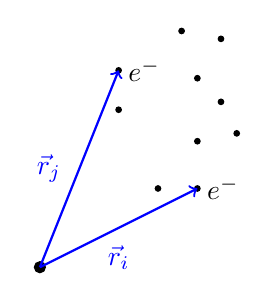
\begin{tikzpicture}
			\filldraw[black]	(0, 0) circle (2pt);
			\filldraw[black]	(1.5, 1) circle (1pt)
								(1, 2) circle (1pt)
								(1.8, 3) circle (1pt)
								(2, 1.6) circle (1pt)
								(2, 1) circle (1pt) node[right]{$e^-$}
								(2.3, 2.9) circle (1pt)
								(2.5, 1.7) circle (1pt)
								(1, 2.5) circle (1pt) node[right]{$e^-$}
								(2, 2.4) circle (1pt)
								(2.3, 2.1) circle (1pt);

			\draw[->, blue, thick]	(0, 0) to node[below=1mm]{$\vec{r}_i$} (2, 1);
			\draw[->, blue, thick]	(0, 0) to node[left=1mm]{$\vec{r}_j$} (1, 2.5);
		\end{tikzpicture}
	\end{center}
}
We can calculate the Potential enegery as follows:
\begin{align}
	v_i(\vec{r}) &= -e \Phi \\
	&= \sum_{k \neq i}^{}{\int_{V}^{}{\frac{e^2 \abs{\xi_k(\vec{r})}^2}{4\pi \epsilon_0 \abs{\vec{r} - \vec{r}'}}dr'}}
\end{align}
\nt{$\Phi$ is electrostatic potential. Furthermore, $\vec{r}_i$ means it \textbf{belongs} to electron i.}

Now we can solve the one electron problem by:
\begin{align}
	& h(\vec{r})\xi(\vec{r}) = \epsilon \xi(\vec{r}) \\
	\Rightarrow & \quad h(\vec{r}) = -\frac{\hbar^2}{2m_e}\nabla^2 + v(\vec{r}) + \sum{V_{electron - ion}(\vec{r} - \vec{R})}
\end{align}
\par Looking at the last part of $h$ we see that in a lattice, $\vec{R}$ is a lattice vector. Then for a solid, the lattice is infinite and therefore $V_{electron - ion}$ will be periodic.
We will call $\sum{V_{electron - ion}(\vec{r} - \vec{R})}$ a periodic potential: $U(\vec{r}) = U(\vec{r} - \vec{R}_l')$ \\ \par
\cor{Conslusion}{As show above we can now write the Schrödinger equation as a simplified wave function:
	\begin{equation}
		\left(-\frac{\hbar^2}{2m_e}\nabla^2 + V(\vec{r})\right)\xi(\vec{r}_i) = \epsilon \xi(\vec{r}_i)
	\end{equation}
}

